%% Overleaf			
%% Software Manual and Technical Document Template	
%% 									
%% This provides an example of a software manual created in Overleaf.

\documentclass{ol-softwaremanual}

% Packages used in this example
\usepackage{graphicx}  % for including images
\usepackage{microtype} % for typographical enhancements
\usepackage{amsmath}   % for equations and mathematics
\usepackage{hyperref}  % for hyperlinks
\usepackage[portuguese]{babel}
\usepackage[a4paper,top=4.2cm,bottom=4.2cm,left=3.5cm,right=3.5cm]{geometry} % for setting page size and margins
% Custom macros used in this example document

\graphicspath{{img/}}

% Frontmatter data; appears on title page
\title{Manual do Usuário}
\version{1.0}
\author{Gustavo Lopes Rodrigues, Lucas Santiago Oliveira}
\softwarelogo{
\includegraphics[width=8cm]{logo.png}}

\begin{document}

\maketitle

\tableofcontents
\newpage

\section{Introdução}

O 3DOff-Visualizer é um programa para a visualização de 
objetos 3D do tipo .off (Object File Format). A seguir, você verá
como interagir com a sua interface, de forma intuitiva.

\section{Interface}

A baixo está algumas capturas de tela do programa em si, a segunda 
em específico, deixa em destaque os principais elementos 
da interface, e que precisam de maior explicação

\begin{figure}[ht]
    \centering
    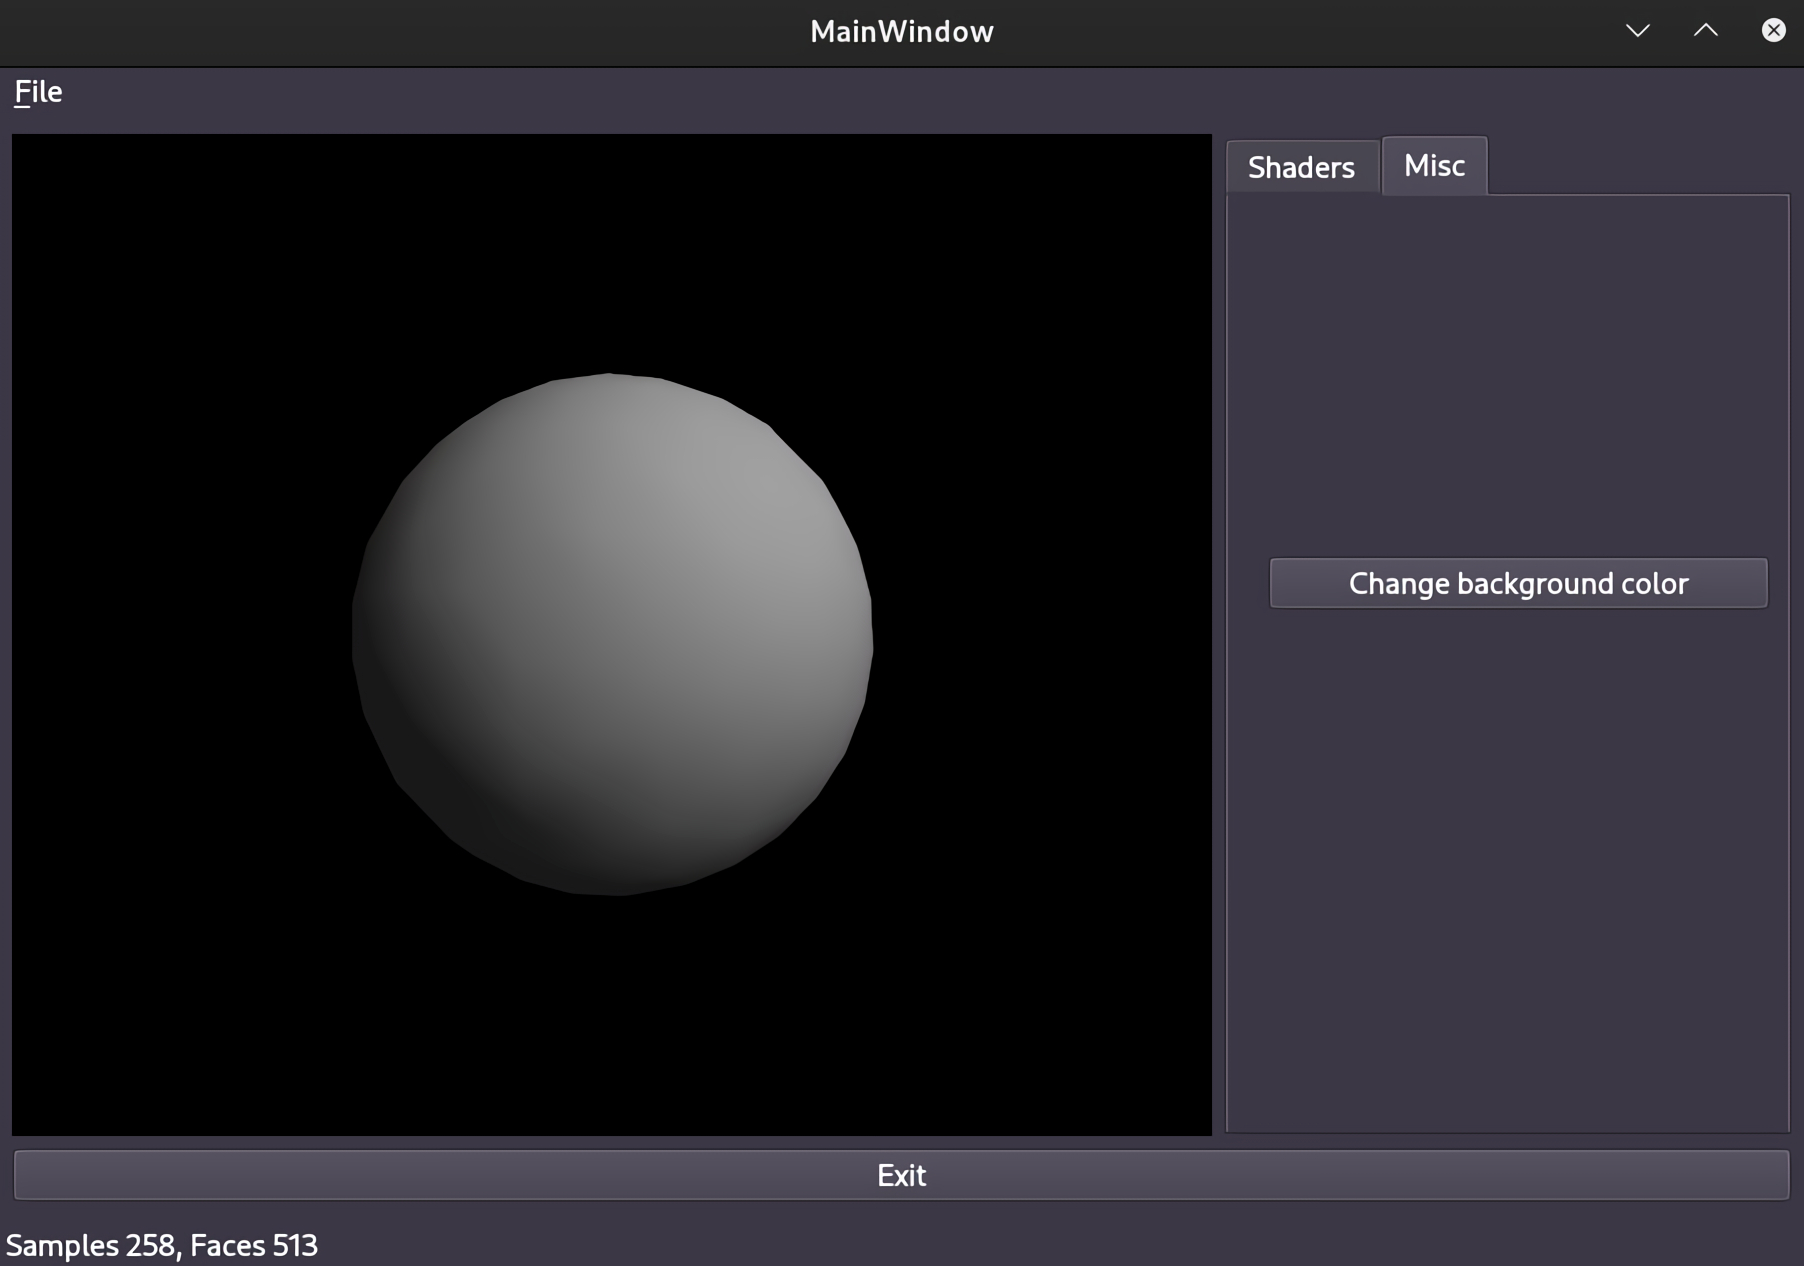
\includegraphics[width=.7\textwidth]{Interface.jpg}
    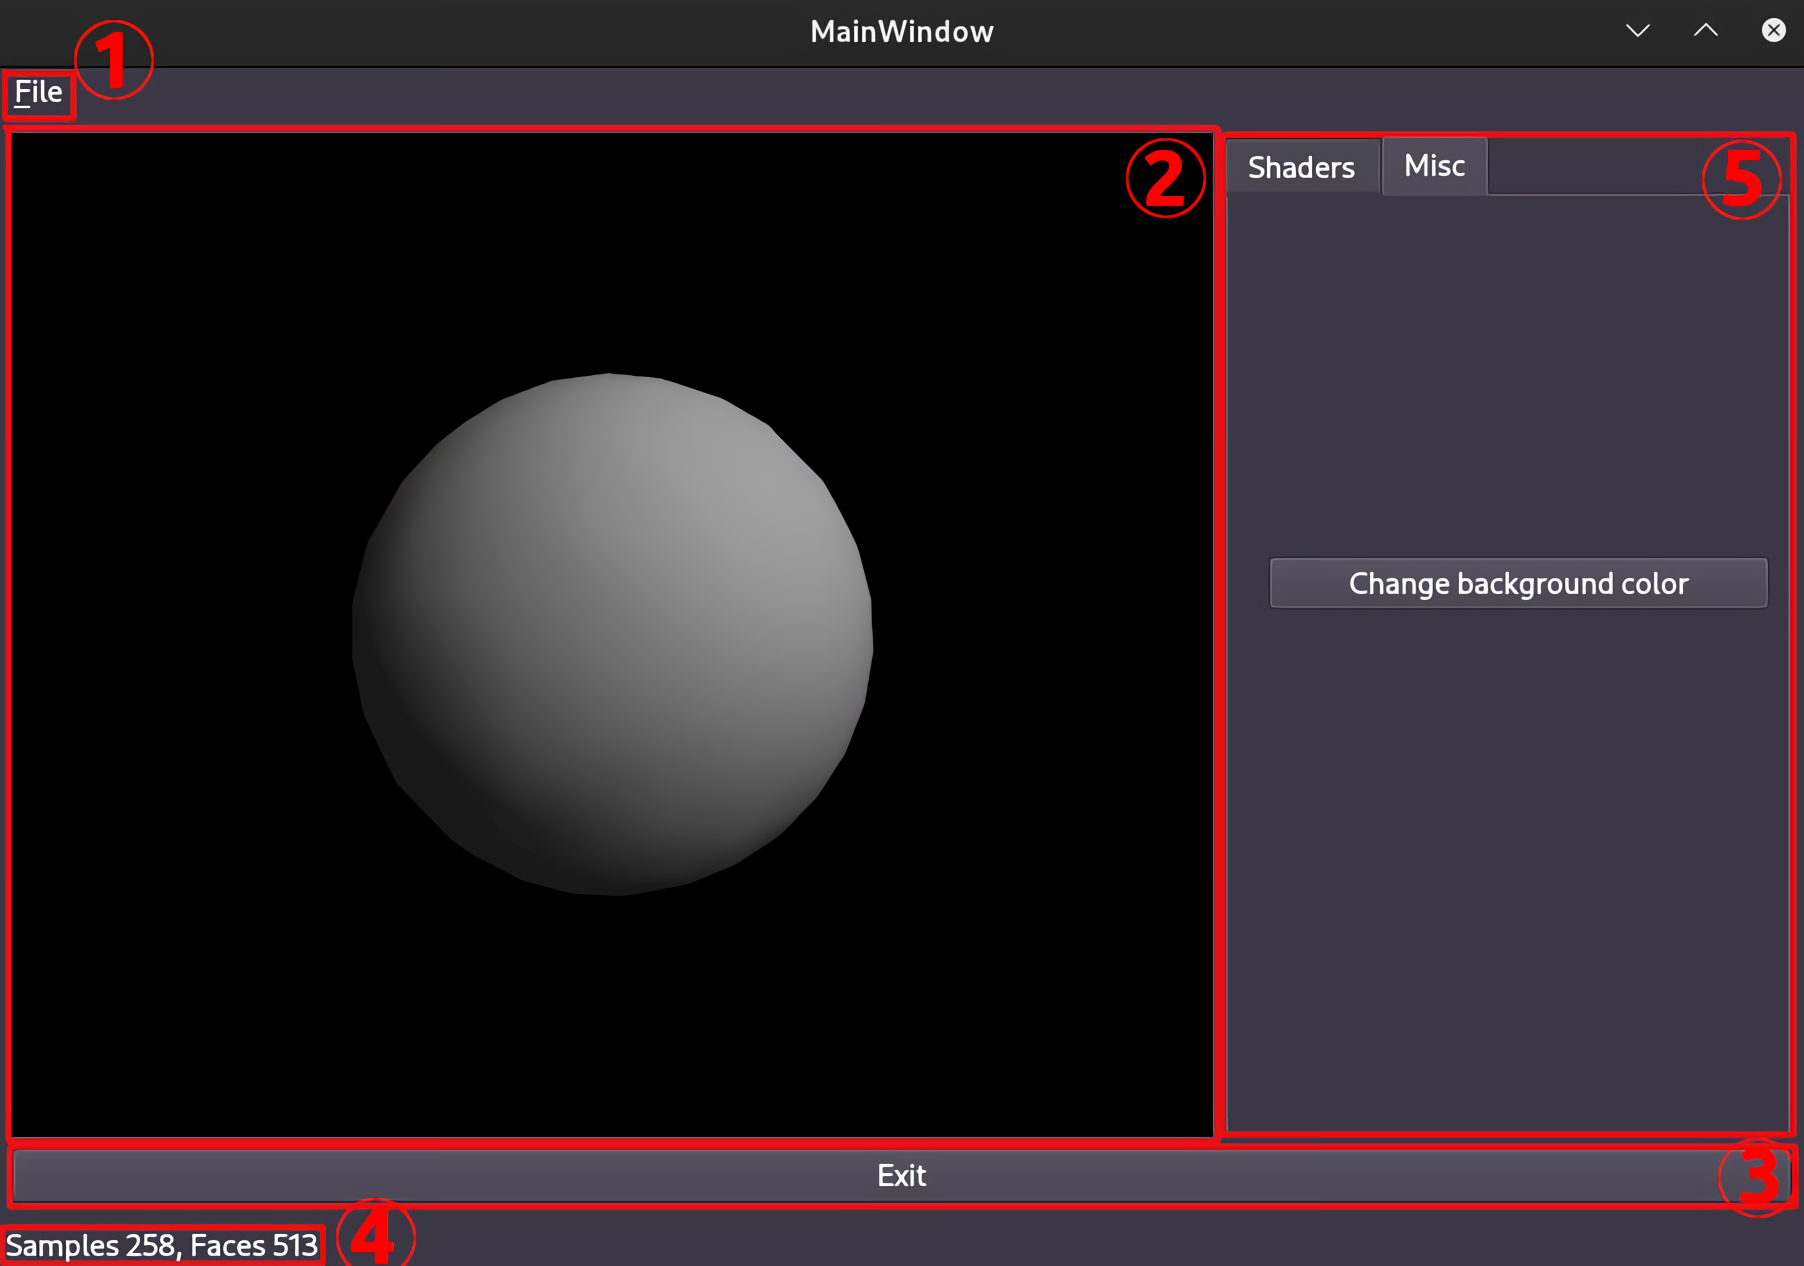
\includegraphics[width=.7\textwidth]{Interfacemarcada.jpg}
\end{figure}

\subsection{File}

Esse botão exibe duas funcionalidades, abrir um arquivo para 
leitura, e fazer uma captura de tela do estado atual do visualizador. 

\subsection{Visualizador}

A principal parte do programa, é onde os objetos 3D após 
serem carregados, seram exibidos para edição e manipulação

\subsection{Sair}

Botão rápido para fechar o programa 

\subsection{Barra de status}

Essa parte da interface serve especificamente para 
informar ao usuário o número de samples e faces que foram 
carregados do objeto 3D após sua leitura.

\subsection{Aba de edição}

Esta região da interface tem o propósito de guardar 
duas abas, com algumas ferramentas adicionais para edição 
do visualizador do objeto. 

\section{Keybinds}

\begin{itemize}
    \item Alt + f $\rightarrow$ abrir o \textbf{File} 
    \begin{itemize}
        \item Alt + f + o $\rightarrow$ abrir um arquivo 
        \item Alt + f + s $\rightarrow$ salvar uma captura de tela 
    \end{itemize}
\end{itemize}

\end{document}
